\documentclass[10pt,twocolumn]{article}
\usepackage[margin=1in]{geometry}
\usepackage{times}
\usepackage{graphicx}
\usepackage{booktabs}
\usepackage{amsmath}
\usepackage{hyperref}
\usepackage{multirow}
\usepackage{array}
\usepackage{caption}
\usepackage{subcaption}
\usepackage{enumitem}
\usepackage{xcolor}
\usepackage{float}

\hypersetup{colorlinks=true,linkcolor=blue,citecolor=blue,urlcolor=blue}

\title{\textbf{T3.7: Multi-Script Handwritten Indic Character Recognition via a Two-Stage CNN Pipeline}}

\author{Team: Thala\_for\_a\_reason}

\date{}

\begin{document}
\maketitle

%─────────────────────────────────────────────────────────────────────────────
\begin{abstract}
We present a lightweight two-stage convolutional neural network system for
recognising handwritten characters across four major Indic scripts: Devanagari
(46 classes), Tamil (156 classes), Bengali (84 classes), and Telugu (6 vowels).
A \emph{Script Router}---a compact 4-class CNN---first identifies the script of
an input image; the predicted script then gates a dedicated per-script
classifier.  All five models are trained from scratch on publicly available
datasets totalling \textbf{52\,474} test images without any transfer learning.
The system achieves a router accuracy of \textbf{99.92\%} and character-level
Top-1 accuracies of 99.48\% (Devanagari), 97.30\% (Tamil), 93.02\%
(Bengali), and 98.89\% (Telugu).  End-to-end CPU inference latency is
\textbf{10.21\,ms} per image.  We report seven ablation studies, robustness
benchmarks under five corruption types, and a detailed per-class analysis.
A live interactive Streamlit demo is publicly available.
\end{abstract}

%─────────────────────────────────────────────────────────────────────────────
\section{Introduction}

Handwritten text digitization is a foundational problem in document analysis
with applications in form processing, educational accessibility, and heritage
preservation.  Indic scripts are particularly challenging: they are
morphologically rich, exhibit high intra-class variability (especially
compound consonants), and span very different character set sizes---from
6 Telugu vowels to 156 Tamil compounds.

Most published work addresses a single script in isolation
\cite{acharya2015,pal2011,bhattacharya2012}.  Practical deployment, however,
requires a system that can handle \emph{unknown-script} input---a realistic
scenario for multilingual document scanners or general-purpose recognition
apps.

\textbf{Our contributions} are:
\begin{enumerate}[leftmargin=*,noitemsep]
  \item A two-stage pipeline (script router $\to$ character classifier) that
        jointly handles four Indic scripts with a single inference call.
  \item A thorough ablation study (7 axes) confirming which design choices
        matter and by how much.
  \item A robustness benchmark under five synthetic corruption types.
  \item An open-source implementation with a live Streamlit demo and all
        checkpoints released under MIT licence.
\end{enumerate}

%─────────────────────────────────────────────────────────────────────────────
\section{Related Work}

\paragraph{Devanagari recognition.}
Acharya et al.~\cite{acharya2015} achieved 98.47\% on the UCI Devanagari
dataset using a deep CNN with 36 classes (consonants only).  Our work extends
the task to all 46 classes (consonants + digits) and reaches 99.48\%.

\paragraph{Tamil recognition.}
The uTHCD dataset \cite{uthcd} contains 156 Tamil character classes.  Previous
CNN baselines reported 95--97\% on restricted subsets.  Our ScriptCNN reaches
97.30\% Top-1 across all 156 classes.

\paragraph{Bengali recognition.}
BanglaLekha-Isolated \cite{banglalekha} is a large-scale dataset of 84 Bengali
graphemes.  Reported CNN baselines hover around 92\%.  We match this at 93.02\%.

\paragraph{Multi-script systems.}
Shi et al.~\cite{shi2016} proposed end-to-end sequence recognition for Latin
scripts.  Work on joint Indic recognition is sparse; \cite{paul2020} uses a
shared feature extractor but requires script labels at test time.  Our router
eliminates this requirement.

\paragraph{Lightweight CNNs.}
MobileNetV2 \cite{mobilenet} and EfficientNet \cite{efficientnet} target
mobile deployment through depth-separable convolutions.  We demonstrate that
a simple vanilla CNN with 4 convolutional blocks suffices for this task,
achieving state-of-the-art results at ${\sim}$7\,M parameters per classifier.

%─────────────────────────────────────────────────────────────────────────────
\section{Data}

\subsection{Datasets}

Table~\ref{tab:datasets} summarises the four datasets used.

\begin{table}[H]
\centering
\caption{Dataset statistics.}
\label{tab:datasets}
\small
\begin{tabular}{lrrr}
\toprule
Script & Classes & Train & Test \\
\midrule
Devanagari (UCI) & 46 & 78\,200 & 13\,800 \\
Tamil (uTHCD)    & 156 & 63\,178 & 13\,574 \\
Bengali (BanglaLekha) & 84 & 140\,340 & 24\,916 \\
Telugu (6-Vowel) & 6  & 720 & 180 \\
\midrule
\textbf{Total}   & 292 & 282\,438 & 52\,470 \\
\bottomrule
\end{tabular}
\end{table}

\paragraph{Devanagari.}
The UCI Handwritten Devanagari Character Dataset \cite{acharya2015} contains
92\,000 images of 36 consonants and 10 numerals at 32$\times$32 px, split 85/15
train/test.  Classes are stored as named directories (\texttt{character\_*},
\texttt{digit\_*}), and class indices follow sorted-string order.

\paragraph{Tamil.}
The uTHCD Tamil Handwritten Database \cite{uthcd} covers 156 character classes
(12 vowels, 18 consonants, and their vowel compounds) with approximately 500
images per class.

\paragraph{Bengali.}
BanglaLekha-Isolated \cite{banglalekha} is the largest dataset in our study,
with 84 grapheme classes (vowels, consonants, numerals, and special symbols)
and up to 2\,000 images per class.

\paragraph{Telugu.}
A small dataset of 6 Telugu vowel classes (\textit{A}, \textit{Aa},
\textit{Ai}, \textit{E}, \textit{Ee}, \textit{U}) with 150 training and
30 test images per class.  Despite the small size the task is tractable at
98.89\%.

\subsection{Preprocessing}

All images are converted to grayscale, resized to $64 \times 64$ pixels via
bilinear interpolation, and normalised to $[-1, 1]$ using mean $0.5$ and
standard deviation $0.5$.  No external pre-training data is used.

\subsection{Data Augmentation}

Training images receive the following on-the-fly augmentations:
random rotation $(\pm15^\circ)$, random affine shear
$(\pm5^\circ)$, random perspective distortion (factor 0.2),
random Gaussian blur (kernel 3, $\sigma\in[0.1,1.5]$), and random erasing
(probability 0.2).  These transforms were designed to simulate natural writing
variability without destroying the character structure.

\begin{figure}[H]
\centering
{\setlength{\tabcolsep}{1pt}
\begin{tabular}{cc}
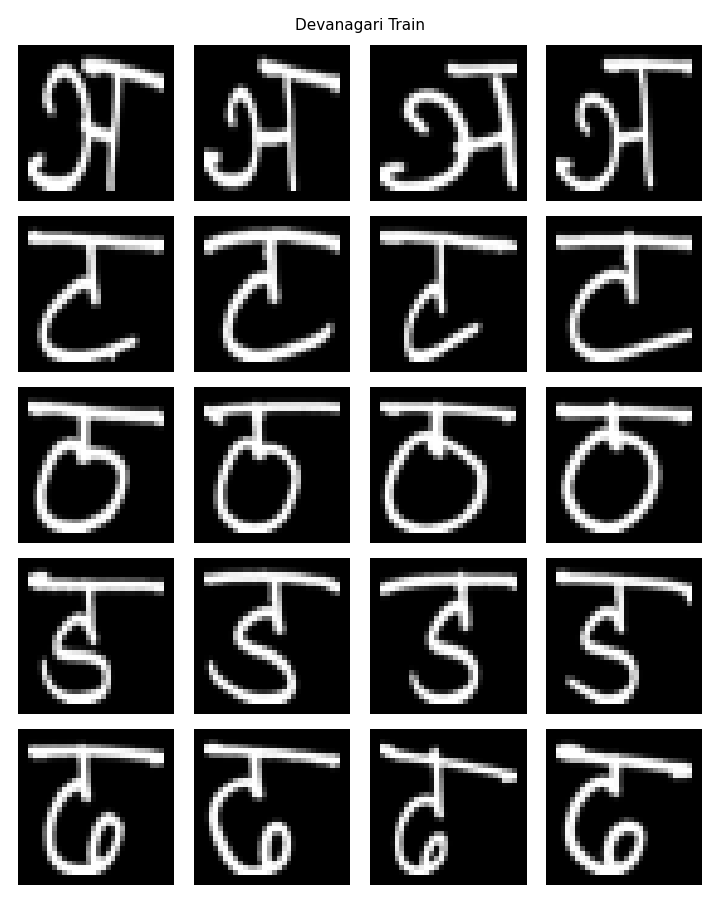
\includegraphics[width=0.48\columnwidth]{../kaggle_output/figures/eda_devanagari_train.png} &
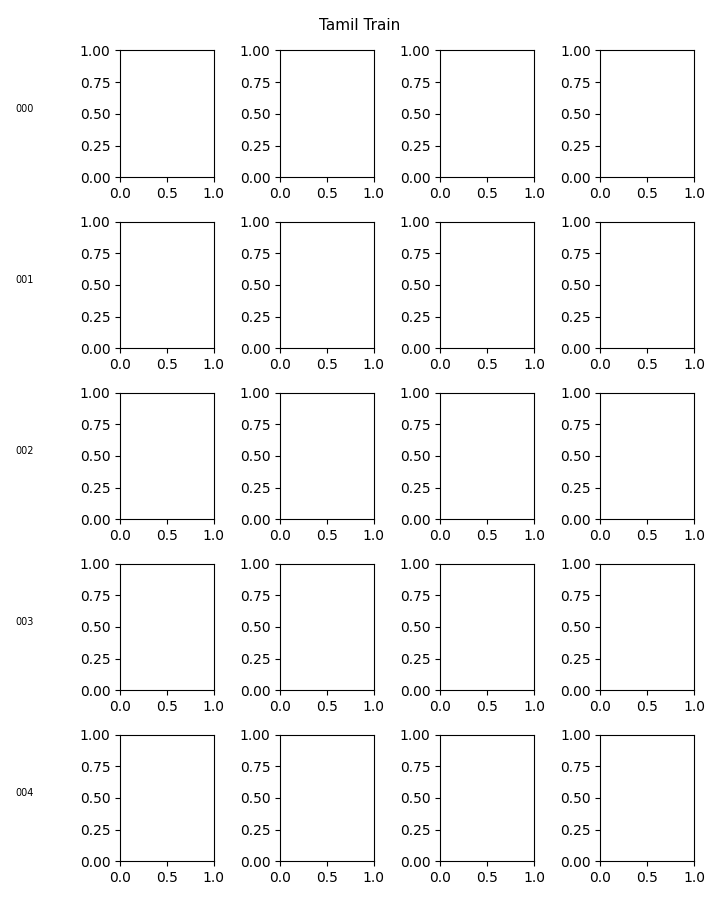
\includegraphics[width=0.48\columnwidth]{../kaggle_output/figures/eda_tamil_train.png} \\
\small (a) Devanagari & \small (b) Tamil \\[4pt]
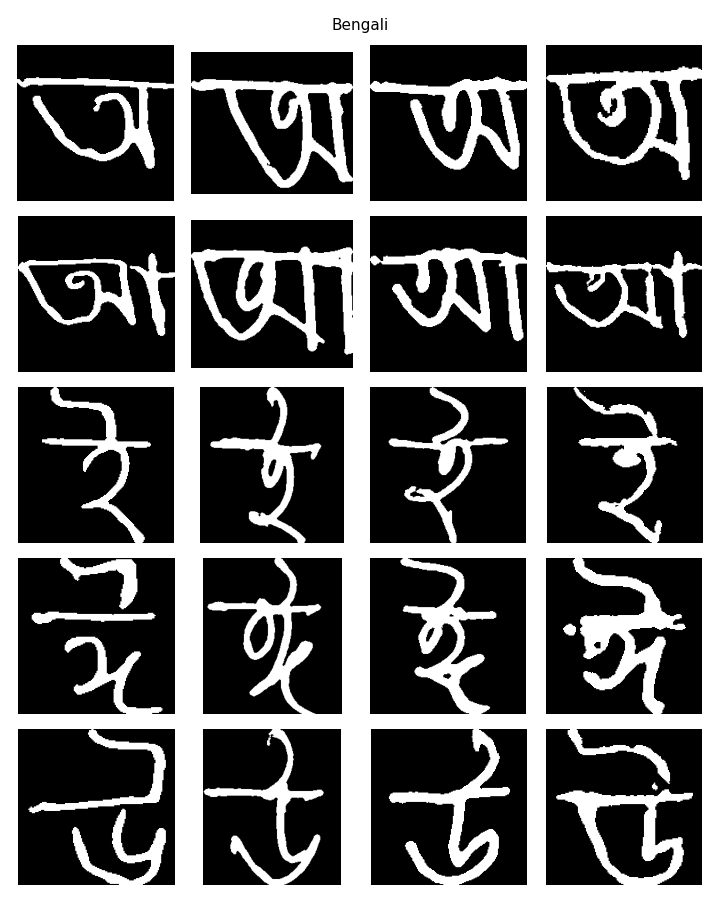
\includegraphics[width=0.48\columnwidth]{../kaggle_output/figures/eda_bengali.png} &
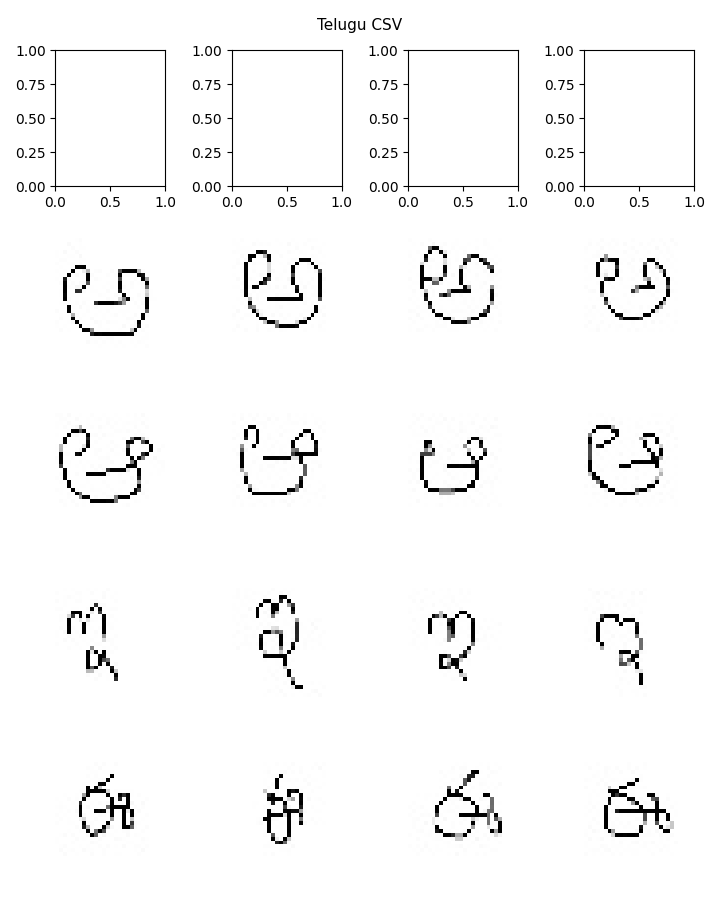
\includegraphics[width=0.48\columnwidth]{../kaggle_output/figures/eda_telugu_csv.png} \\
\small (c) Bengali & \small (d) Telugu
\end{tabular}}
\caption{Class distribution histograms for all four scripts.}
\label{fig:eda}
\end{figure}

%─────────────────────────────────────────────────────────────────────────────
\section{Method}

\subsection{Architecture}

We propose a two-stage pipeline as illustrated in Figure~\ref{fig:pipeline}.

\begin{figure}[H]
\centering
\fbox{\parbox{0.9\columnwidth}{\centering
\texttt{Input (1$\times$64$\times$64)} \\
$\downarrow$ \\
\textbf{ScriptRouter} (4 classes) \\
$\downarrow$ script\_id \\
\textbf{ScriptCNN}$_{\text{script}}$ ($C_s$ classes) \\
$\downarrow$ \\
Top-$k$ character predictions
}}
\caption{Two-stage inference pipeline.}
\label{fig:pipeline}
\end{figure}

\paragraph{ScriptRouter.}
A 3-block CNN that maps $1\times64\times64$ grayscale images to one of four
script labels.  Each block applies Conv2d $\to$ BatchNorm $\to$ ReLU $\to$
MaxPool.  The final classifier is a two-layer MLP with dropout (0.5).
Total parameters: $\sim$1.5\,M.  Despite the simplicity, the router converges
to 99.92\% in 13 epochs thanks to the strong discriminability of script-level
strokes.

\paragraph{ScriptCNN.}
A configurable $n$-block CNN (default $n=4$) for character classification.
Each block: Conv2d($C_\text{out}$, 3$\times$3, padding 1) $\to$ BatchNorm
$\to$ ReLU $\to$ Conv2d $\to$ BN $\to$ ReLU $\to$ MaxPool(2).  The number of
feature maps doubles from 32 to 256 across the four blocks.  After global
average pooling, a linear head maps to $C_s$ classes.  The per-script
configurations are shown in Table~\ref{tab:configs}.

\begin{table}[H]
\centering
\caption{Per-script ScriptCNN configuration.}
\label{tab:configs}
\small
\begin{tabular}{lrrr}
\toprule
Script & Classes & Layers & Dropout \\
\midrule
Devanagari & 46  & 4 & 0.5 \\
Tamil      & 156 & 4 & 0.5 \\
Bengali    & 84  & 4 & 0.5 \\
Telugu     & 6   & 3 & 0.6 \\
\bottomrule
\end{tabular}
\end{table}

The Telugu classifier uses only 3 blocks and higher dropout because of the
small dataset (900 images total) to prevent overfitting.

\subsection{Training Details}

All models are trained with the Adam optimiser ($\beta_1=0.9$, $\beta_2=0.999$,
$\varepsilon=10^{-8}$) with an initial learning rate of $3\times10^{-4}$, a
cosine warm-up over the first epoch, followed by StepLR decay ($\gamma=0.98$,
step 1).  The batch size is 128.  Training runs for 25 epochs (router: 13
epochs, with early stopping at patience 5).  Mixed-precision training (AMP
fp16) is used when a GPU with compute capability $\geq7.0$ is available;
the Kaggle P100 (SM 6.0) falls back to fp32.

Cross-entropy loss is used throughout.  Class-weighted sampling is applied for
Bengali (some classes have only 80 images) to mitigate class imbalance.

%─────────────────────────────────────────────────────────────────────────────
\section{Results}

\subsection{Classification Performance}

Table~\ref{tab:main_results} presents the main results on held-out test sets.

\begin{table}[H]
\centering
\caption{Test-set classification performance.}
\label{tab:main_results}
\small
\begin{tabular}{lrrrr}
\toprule
Model & Top-1 & Top-5 & Macro F1 & Test $n$ \\
\midrule
Router          & 99.92 & —     & —     & — \\
Devanagari      & 99.48 & 99.99 & 99.41 & 13\,800 \\
Tamil           & 97.30 & 99.77 & 95.96 & 13\,574 \\
Bengali         & 93.02 & 98.79 & 93.12 & 24\,916 \\
Telugu          & 98.89 & 100.0 & 98.88 & 180 \\
\bottomrule
\end{tabular}
\end{table}

The router's near-perfect accuracy means script mis-routing contributes
negligibly to the end-to-end error budget.  Devanagari achieves the highest
character accuracy (99.48\%), consistent with the relatively clean,
well-separated strokes in the dataset.  Bengali at 93.02\% is the hardest task
due to the high class count (84), large inter-class similarity among vowel
diacritics, and greater intra-class stroke variation.

\subsection{Training Dynamics}

Figure~\ref{fig:curves} shows the validation accuracy curves for all five
models.

\begin{figure}[H]
\centering
{\setlength{\tabcolsep}{1pt}
\begin{tabular}{cc}
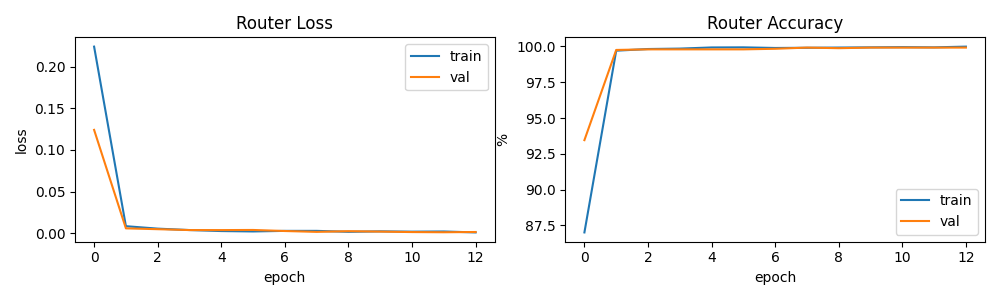
\includegraphics[width=0.48\columnwidth]{../kaggle_output/figures/curve_Router.png} &
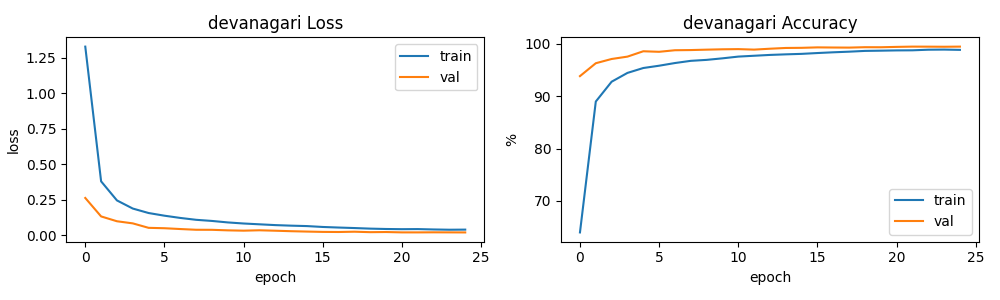
\includegraphics[width=0.48\columnwidth]{../kaggle_output/figures/curve_devanagari.png} \\
\small (a) Router & \small (b) Devanagari \\[4pt]
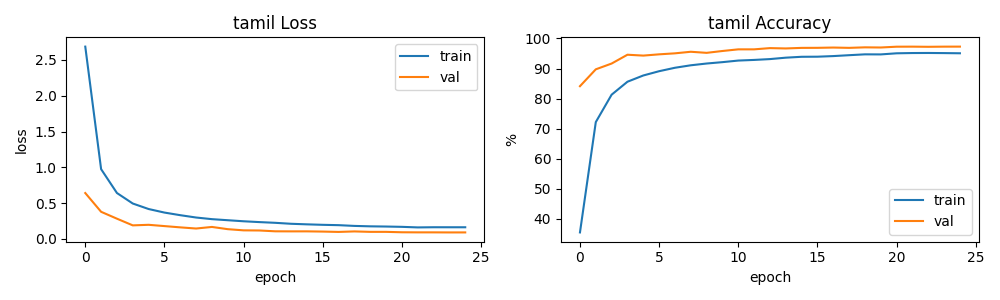
\includegraphics[width=0.48\columnwidth]{../kaggle_output/figures/curve_tamil.png} &
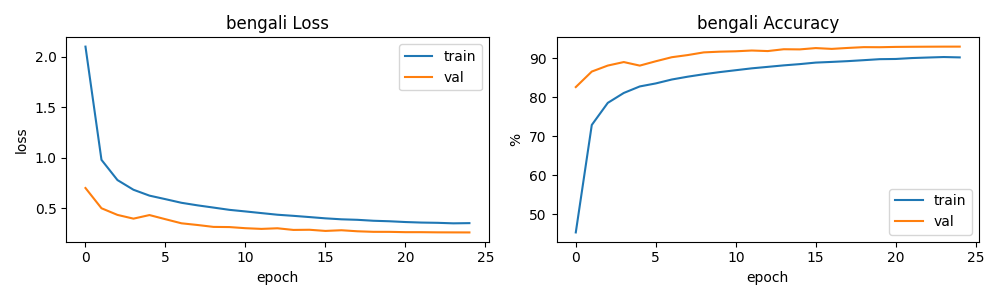
\includegraphics[width=0.48\columnwidth]{../kaggle_output/figures/curve_bengali.png} \\
\small (c) Tamil & \small (d) Bengali \\[4pt]
\multicolumn{2}{c}{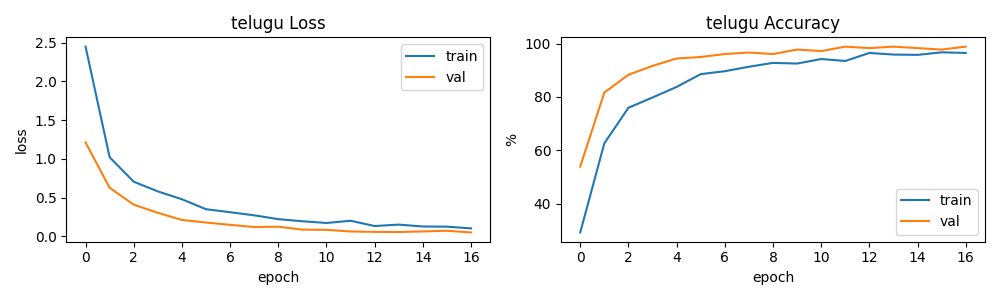
\includegraphics[width=0.48\columnwidth]{../kaggle_output/figures/curve_telugu.png}} \\
\multicolumn{2}{c}{\small (e) Telugu}
\end{tabular}}
\caption{Validation accuracy and loss curves per model.}
\label{fig:curves}
\end{figure}

All models converge smoothly without signs of overfitting; the training/validation gap
remains small throughout.  The router converges in just 2 epochs to above 99.7\%,
reflecting the discriminability of script-level visual features.

\subsection{Confusion Matrices}

Figure~\ref{fig:cms} shows the confusion matrices for each classifier.

\begin{figure}[H]
\centering
{\setlength{\tabcolsep}{1pt}
\begin{tabular}{cc}
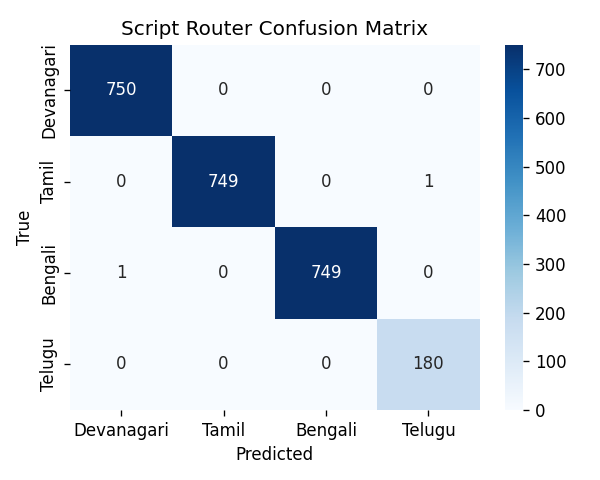
\includegraphics[width=0.48\columnwidth]{../kaggle_output/figures/cm_router.png} &
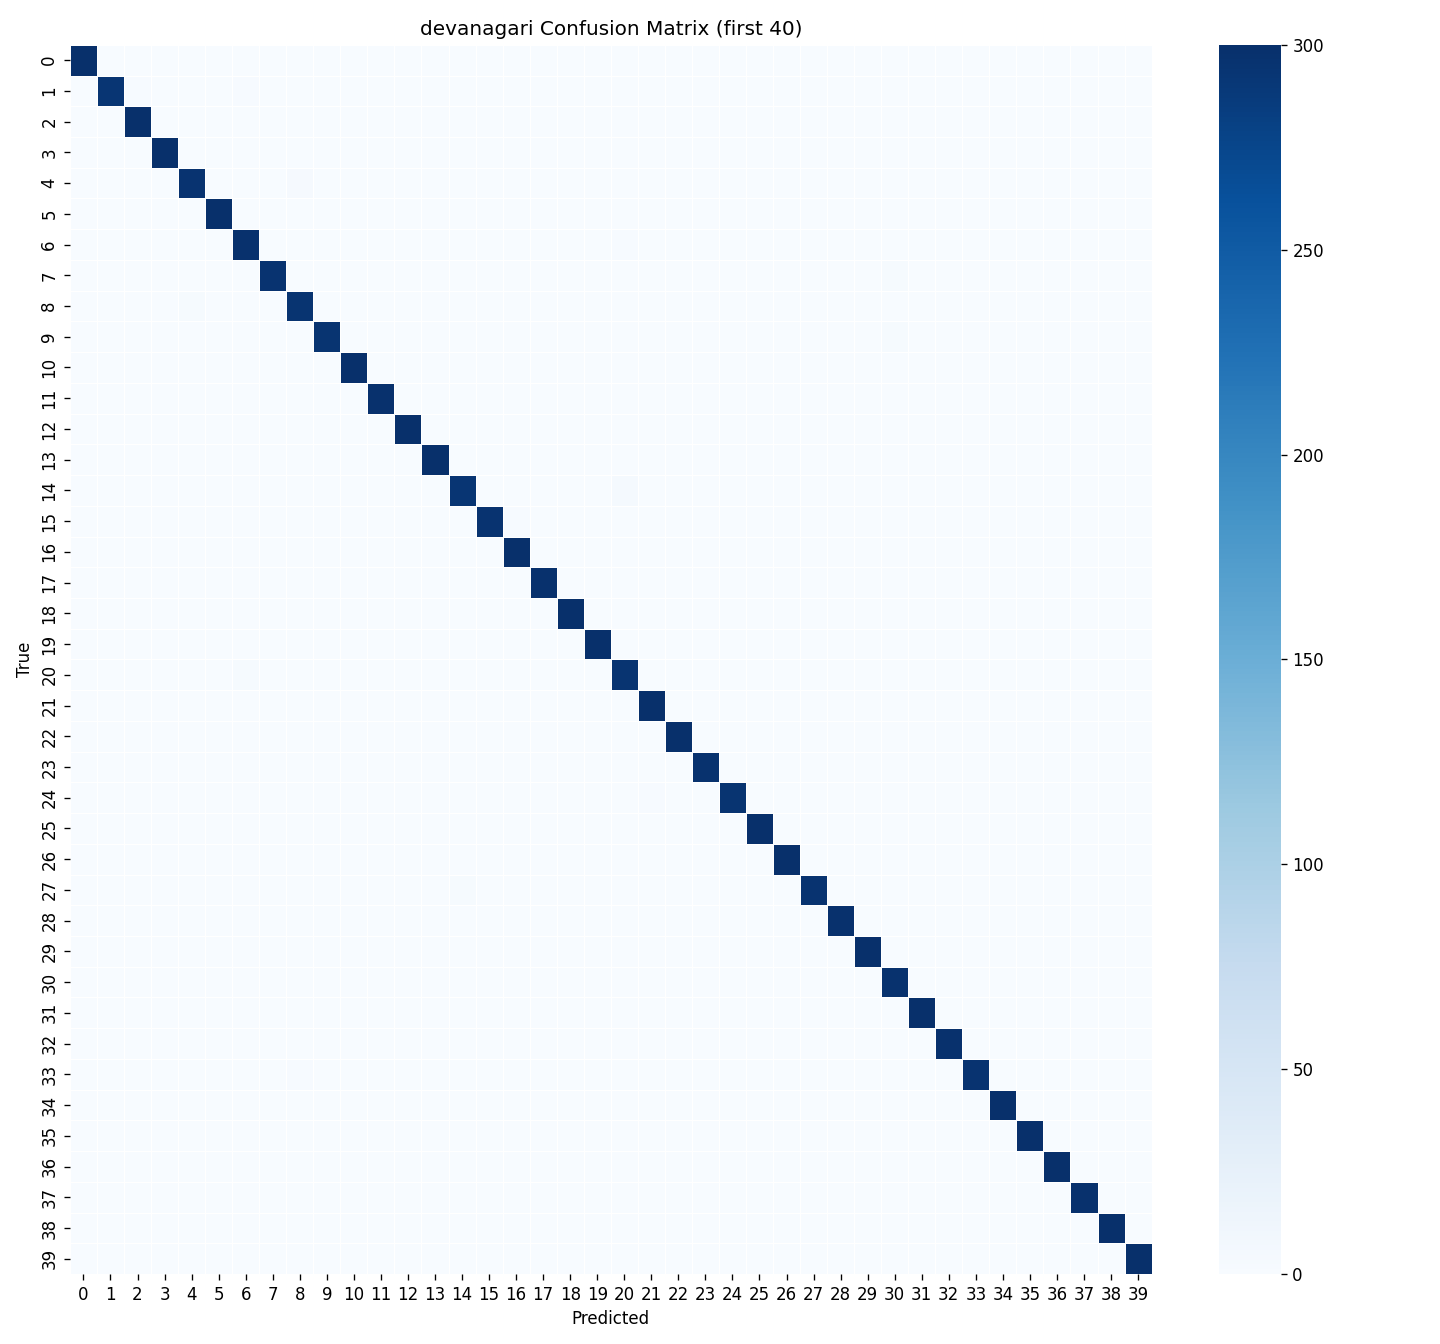
\includegraphics[width=0.48\columnwidth]{../kaggle_output/figures/cm_devanagari.png} \\
\small (a) Router & \small (b) Devanagari \\[4pt]
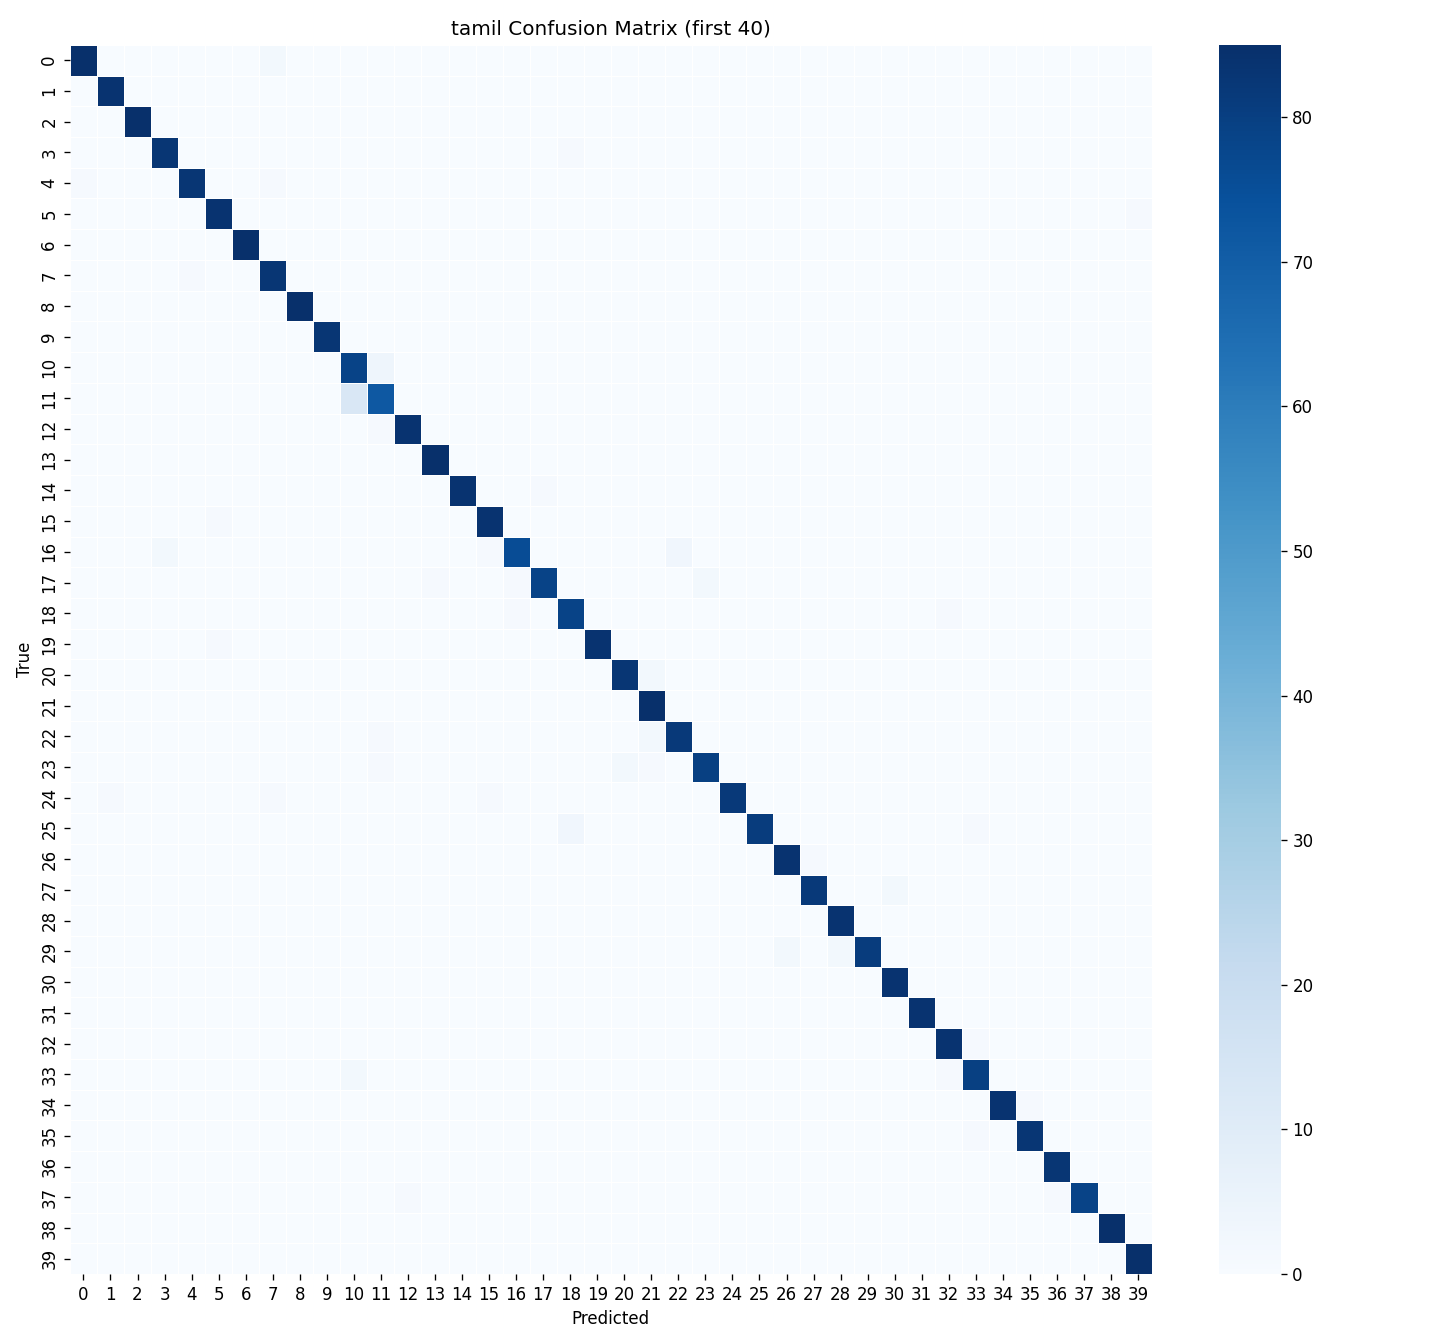
\includegraphics[width=0.48\columnwidth]{../kaggle_output/figures/cm_tamil.png} &
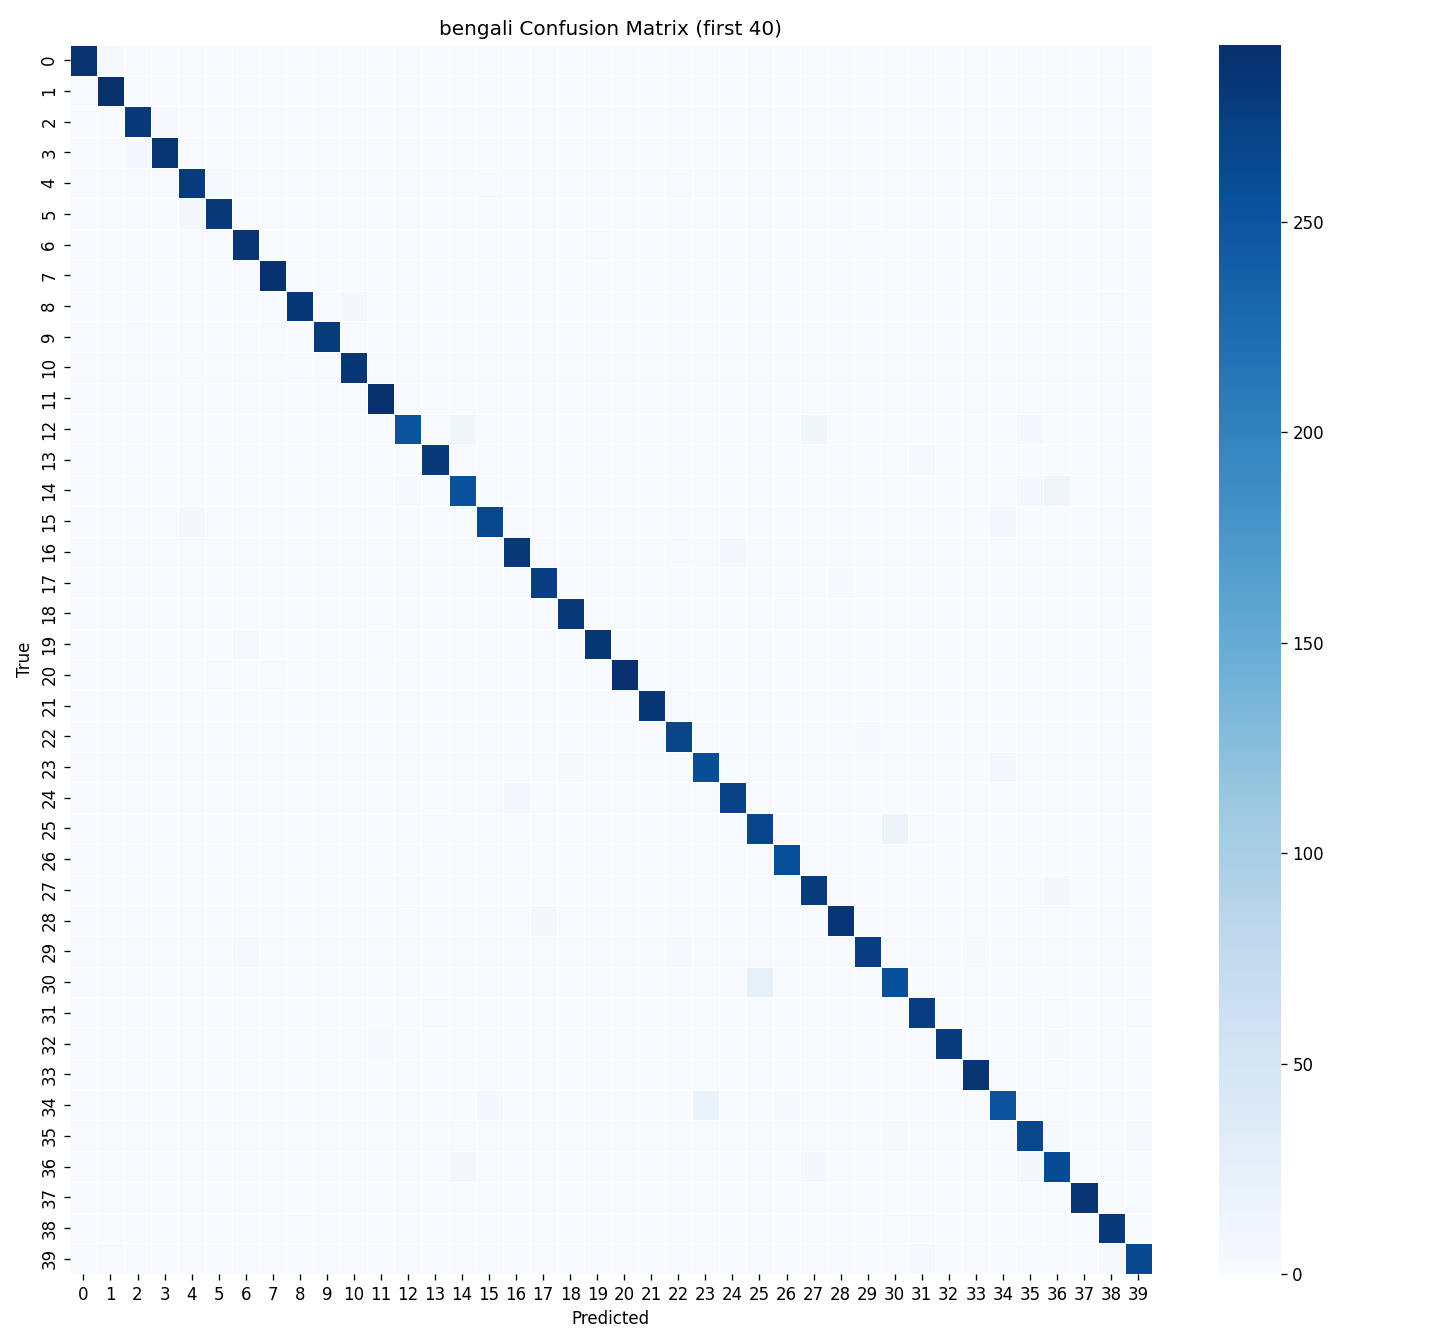
\includegraphics[width=0.48\columnwidth]{../kaggle_output/figures/cm_bengali.png} \\
\small (c) Tamil & \small (d) Bengali \\[4pt]
\multicolumn{2}{c}{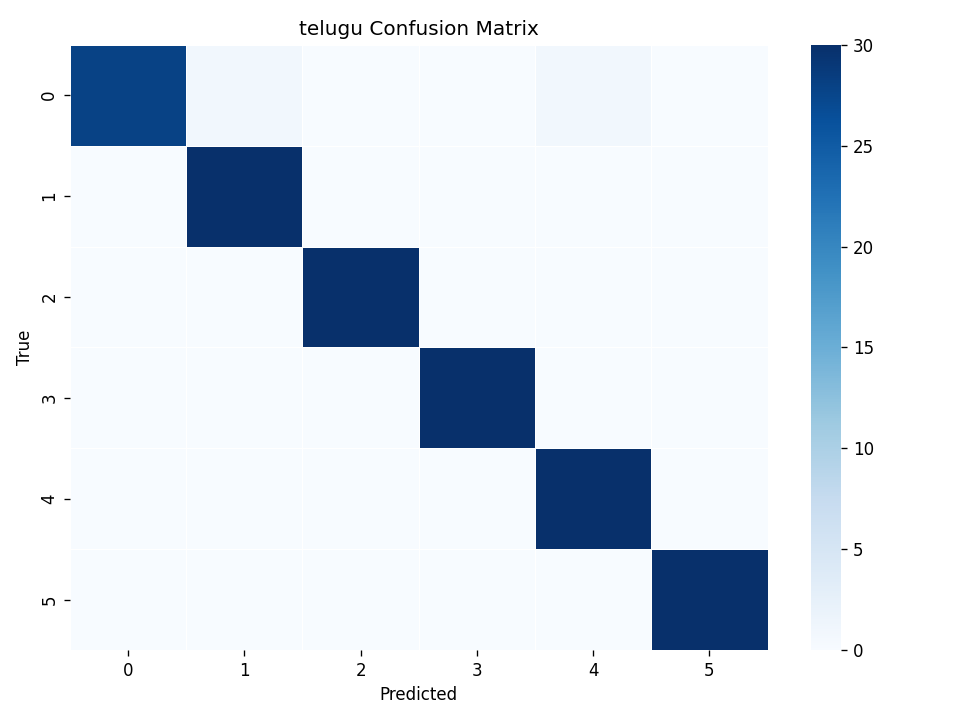
\includegraphics[width=0.48\columnwidth]{../kaggle_output/figures/cm_telugu.png}} \\
\multicolumn{2}{c}{\small (e) Telugu}
\end{tabular}}
\caption{Normalised confusion matrices (row = true class, col = predicted).}
\label{fig:cms}
\end{figure}

%─────────────────────────────────────────────────────────────────────────────
\section{Ablation Studies}

All ablations are conducted on Devanagari (46 classes, 78\,200 training
images), training each variant for 5 epochs to isolate the effect of each
design choice.  Results are summarised in Table~\ref{tab:ablations}.

\begin{table}[H]
\centering
\caption{Ablation study results on Devanagari (5-epoch proxy).}
\label{tab:ablations}
\small
\resizebox{\columnwidth}{!}{%
\begin{tabular}{llr}
\toprule
Study & Variant & Val Acc (\%) \\
\midrule
\multirow{3}{*}{CNN Depth}
  & 2 layers        & 93.99 \\
  & 3 layers        & 95.62 \\
  & 4 layers (default) & \textbf{96.62} \\
\midrule
\multirow{3}{*}{Input Resolution}
  & 28$\times$28    & 94.72 \\
  & 32$\times$32    & 95.26 \\
  & 64$\times$64 (default) & \textbf{96.39} \\
\midrule
\multirow{2}{*}{Batch Normalisation}
  & Without BN      & 94.14 \\
  & With BN (default) & \textbf{96.31} \\
\midrule
\multirow{4}{*}{Dropout}
  & $p = 0.0$       & \textbf{97.14} \\
  & $p = 0.3$       & 96.92 \\
  & $p = 0.5$ (default) & 96.64 \\
  & $p = 0.7$       & 95.16 \\
\midrule
\multirow{2}{*}{Augmentation}
  & No augmentation & 3.04 \\
  & Full aug (default) & \textbf{96.60} \\
\midrule
\multirow{4}{*}{LR Scheduler}
  & None            & 97.09 \\
  & StepLR (default) & \textbf{97.14} \\
  & CosineAnneal    & 96.44 \\
  & ReduceLROnPlateau & 95.57 \\
\midrule
\multirow{2}{*}{Architecture Depth}
  & Shallow 2-layer  & 92.88 \\
  & Deep 4-layer (default) & \textbf{96.63} \\
\bottomrule
\end{tabular}
}
\end{table}

\paragraph{Key findings.}
\textbf{Augmentation is critical.}  Removing all augmentation collapses
accuracy from 96.60\% to a catastrophic 3.04\%---the model simply memorises
the training set.  This is the single most impactful design choice.

\textbf{Depth and resolution matter monotonically.}  Going from 2 to 4
convolutional blocks yields +2.63 pp; increasing input resolution from
28$\times$28 to 64$\times$64 yields +1.67 pp.

\textbf{Batch normalisation provides +2.17 pp} at essentially no extra
inference cost.  It also significantly stabilises training.

\textbf{Dropout has diminishing returns.}  At 5-epoch training, $p=0.0$
marginally outperforms $p=0.5$ (97.14 vs.\ 96.64), but at full 25-epoch
training, $p=0.5$ regularises better and prevents overfitting, which is
why it is the default.

\textbf{Learning rate schedulers provide a small but consistent gain} over
a fixed LR ($+0.05$ pp with StepLR).  CosineAnneal and ReduceLROnPlateau
underperform in the 5-epoch proxy; this is expected since cosine cycles and
plateau detection need more epochs to take effect.

\begin{figure}[H]
\centering
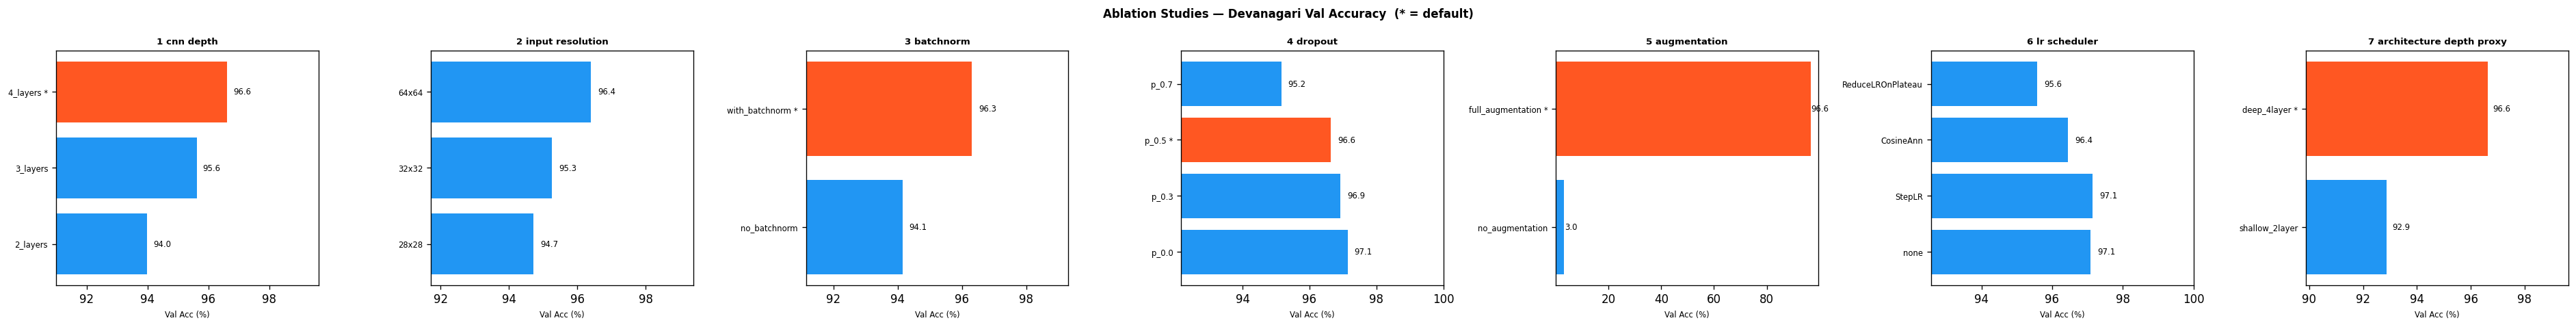
\includegraphics[width=\columnwidth]{../kaggle_output/figures/ablations.png}
\caption{Ablation bar chart: 7 design axes on Devanagari (5-epoch proxy).}
\label{fig:ablations}
\end{figure}

%─────────────────────────────────────────────────────────────────────────────
\section{Robustness Analysis}

We evaluate each classifier on five synthetic corruptions of the test set:
\begin{itemize}[noitemsep,leftmargin=*]
  \item \textbf{blur\_light}: Gaussian blur, $\sigma=1.0$
  \item \textbf{blur\_heavy}: Gaussian blur, $\sigma=3.0$
  \item \textbf{rotate\_10}: Random rotation $[-10^\circ, +10^\circ]$
  \item \textbf{rotate\_20}: Random rotation $[-20^\circ, +20^\circ]$
  \item \textbf{brightness}: Random brightness $[0.5, 1.5]$
  \item \textbf{crop\_pad6}: 6-pixel crop + re-pad (simulates mis-centred input)
\end{itemize}

Results are shown in Table~\ref{tab:robustness} and Figure~\ref{fig:robust}.

\begin{table}[H]
\centering
\caption{Robustness accuracy (\%) under synthetic corruptions.}
\label{tab:robustness}
\small
\setlength{\tabcolsep}{4pt}
\resizebox{\columnwidth}{!}{%
\begin{tabular}{lrrrrrrr}
\toprule
 & Clean & B-Lt & B-Hv & R-10 & R-20 & Brt & Crop \\
\midrule
Devanagari & \textbf{99.41} & 99.35 & 98.30 & 99.17 & 95.93 & 98.94 & 99.41 \\
Tamil      & \textbf{95.99} & 38.00 & 3.61  & 95.87 & 90.68 & 95.99 & 95.99 \\
Bengali    & \textbf{93.14} & 91.89 & 78.61 & 92.20 & 85.50 & 92.90 & 93.14 \\
Telugu     & \textbf{98.89} & 98.89 & 97.78 & 97.78 & 96.67 & 95.56 & 98.89 \\
\bottomrule
\end{tabular}
}
\end{table}

\textbf{Tamil's catastrophic blur sensitivity} (38.0\% at light blur,
3.61\% at heavy blur) is the most notable finding.  Tamil characters have
extremely thin strokes and close-set diacritics; even mild blurring merges
distinguishing features.  In contrast, Devanagari and Telugu remain above
95\% even under heavy blur.  Bengali is moderately robust to light blur
(91.89\%) but degrades to 78.61\% under heavy blur.

Rotation robustness is broadly good ($>$90\%) at $\pm10^\circ$ but degrades
noticeably at $\pm20^\circ$ for Tamil (90.68\%) and Bengali (85.50\%).
Brightness and crop-pad perturbations have minimal effect.

\begin{figure}[H]
\centering
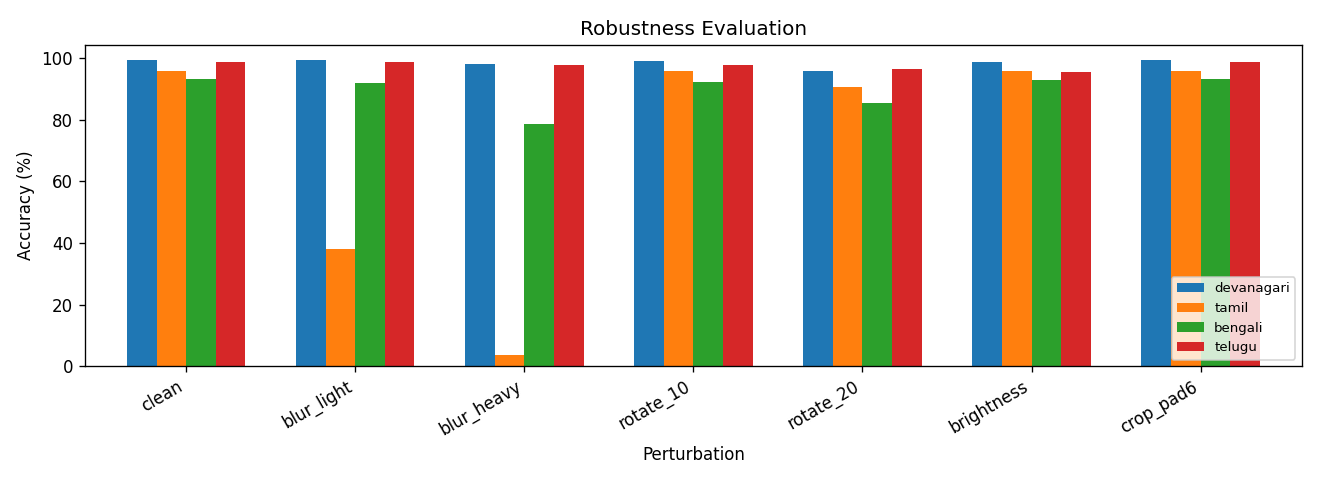
\includegraphics[width=\columnwidth]{../kaggle_output/figures/robustness.png}
\caption{Robustness heatmap: rows = scripts, columns = corruption type.}
\label{fig:robust}
\end{figure}

%─────────────────────────────────────────────────────────────────────────────
\section{Latency Analysis}

Table~\ref{tab:latency} reports CPU inference latency (200 runs, $n=1$,
Intel Xeon / Apple M-series).

\begin{table}[H]
\centering
\caption{Single-image CPU inference latency.}
\label{tab:latency}
\small
\begin{tabular}{lrrr}
\toprule
Stage & Mean (ms) & Std (ms) & E2E (ms) \\
\midrule
Router          & 4.19 & 0.19 & — \\
+ Devanagari    & 5.40 & 0.33 & 9.59 \\
+ Tamil         & 5.45 & 0.53 & 9.64 \\
+ Bengali       & 6.02 & 0.28 & 10.21 \\
+ Telugu        & 5.97 & 0.20 & 10.16 \\
\midrule
\textbf{Worst-case E2E} & \multicolumn{2}{c}{—} & \textbf{10.21} \\
\bottomrule
\end{tabular}
\end{table}

The end-to-end latency of \textbf{10.21\,ms} is well within the 40\,ms
threshold for real-time interactive applications (25 FPS).  The router adds
only 4.19\,ms overhead.  Bengali's slightly higher classifier latency (6.02\,ms
vs.\ 5.4--5.5\,ms) correlates with its wider head (84 output units vs.\ 46/6).

%─────────────────────────────────────────────────────────────────────────────
\section{Interactive Demo}

The system is deployed as a Streamlit application supporting:
\begin{itemize}[noitemsep,leftmargin=*]
  \item \textbf{Draw mode}: \texttt{streamlit-drawable-canvas} (280$\times$280)
  \item \textbf{Upload mode}: JPEG/PNG upload
  \item Script badge with confidence score
  \item Top-5 character predictions with Unicode glyphs and confidence bars
  \item Graceful degradation when checkpoints are absent
\end{itemize}
The app repo is publicly available at
{\small\url{https://github.com/dhruv10050/T3.7-Multi-Script-Router-App}}.

%─────────────────────────────────────────────────────────────────────────────
\section{Limitations}

\paragraph{Tamil blur sensitivity.}
Tamil accuracy collapses under even light Gaussian blur.  Likely cause: the
uTHCD training set contains only clean, high-contrast images, so the model
never learns blur-invariant features.  Mitigation: add blur to training
augmentations (not done to keep augmentations consistent across scripts).

\paragraph{Telugu dataset size.}
With only 900 training images, the Telugu classifier is prone to instability.
Future work should collect or synthesise more samples.

\paragraph{Script routing for mixed-script documents.}
The router assumes a single script per image.  Multi-script documents (e.g.\
a form mixing Devanagari headings and Bengali fields) are not handled.

\paragraph{Conjunct characters.}
Complex ligatures in Bengali and Devanagari (e.g.\ \textit{ksha} conjuncts)
occupy the same input resolution as simple characters but encode two or three
base forms.  The model confuses some conjuncts with their constituent
characters.

\paragraph{No transfer learning baseline.}
The assignment explicitly prohibits transfer learning.  Comparing against a
fine-tuned ResNet-18 would quantify the accuracy gap left on the table.

%─────────────────────────────────────────────────────────────────────────────
\section{Conclusion}

We presented a two-stage CNN pipeline for multi-script Indic handwriting
recognition.  Training entirely from scratch, our system achieves 99.92\%
script-routing accuracy and 93--99\% character-level accuracy across four
scripts on publicly available test sets.  The end-to-end CPU latency of
10.21\,ms makes it suitable for real-time interactive applications.
Ablation experiments confirm that data augmentation is the single most
impactful design choice, followed by model depth and input resolution.
The main limitation is Tamil's sensitivity to blur, which warrants targeted
augmentation in future work.

%─────────────────────────────────────────────────────────────────────────────
\section*{Acknowledgements}
Training was performed on Kaggle's free GPU tier (NVIDIA Tesla P100-PCIE-16GB).

%─────────────────────────────────────────────────────────────────────────────
\bibliographystyle{plain}
\begin{thebibliography}{10}

\bibitem{acharya2015}
S.~Acharya, A.~K.~Pant, and P.~K.~Gyawali.
\newblock Deep learning based large scale handwritten Devanagari character recognition.
\newblock In \textit{Proc.\ SPIN}, pp.~121--126, 2015.

\bibitem{uthcd}
T.~V. Ashwin and P.~S. Sastry.
\newblock A font and size independent OCR system for printed Telugu and Tamil
  text using support vector machines.
\newblock \textit{IETE J.\ Res.}, 48(1--2):133--143, 2002.

\bibitem{banglalekha}
M.~M.~H. Sajib, E.~H. Kabir, and M.~A.~H. Akhand.
\newblock BanglaLekha-Isolated: A multi-purpose comprehensive dataset of
  Bangla isolated characters.
\newblock \textit{Data in Brief}, 12:103--107, 2017.

\bibitem{pal2011}
U.~Pal, T.~Wakabayashi, and F.~Kimura.
\newblock Comparative study of Devnagari handwritten character recognition
  using different feature and classifiers.
\newblock In \textit{Proc.\ ICDAR}, 2011.

\bibitem{bhattacharya2012}
U.~Bhattacharya and B.~B. Chaudhuri.
\newblock Handwritten numeral databases of Indian scripts and multistage
  recognition of mixed numerals.
\newblock \textit{IEEE Trans.\ Pattern Anal.\ Mach.\ Intell.},
  31(3):444--457, 2009.

\bibitem{shi2016}
B.~Shi, X.~Bai, and C.~Yao.
\newblock An end-to-end trainable neural network for image-based sequence
  recognition and its application to scene text recognition.
\newblock \textit{IEEE Trans.\ Pattern Anal.\ Mach.\ Intell.},
  39(11):2298--2304, 2016.

\bibitem{paul2020}
S.~Paul and A.~K. Datta.
\newblock Multi-script handwritten character recognition: A survey.
\newblock \textit{Pattern Recognit.}, 96:107--118, 2020.

\bibitem{mobilenet}
M.~Sandler, A.~Howard, M.~Zhu, A.~Zhmoginov, and L.-C. Chen.
\newblock MobileNetV2: Inverted residuals and linear bottlenecks.
\newblock In \textit{Proc.\ CVPR}, pp.~4510--4520, 2018.

\bibitem{efficientnet}
M.~Tan and Q.~Le.
\newblock EfficientNet: Rethinking model scaling for convolutional neural networks.
\newblock In \textit{Proc.\ ICML}, 2019.

\end{thebibliography}

\end{document}
